\documentclass[a4paper,12pt]{article}
\usepackage{anysize}
\marginsize{3cm}{3cm}{1cm}{3cm}
\usepackage{amsmath}
\usepackage{amsthm}
\usepackage{bbm}
\usepackage{graphicx}

\begin{document}
\title{\textbf{Computational Statistics: Homework 1}}
\author{Michal Porvaznik \\ Nemesis key = 9cfd313}
\date{March 1, 2015}
\maketitle
%
\section*{Exercise 1}
%
\begin{center}
    \begin{tabular}{| l | l | p{5 cm} |}
    \hline
    Function & Transforamtion & Linear form \\ \hline
    $y = \alpha x^{\beta}$ & $y' = log(y)$, $x' = log(x)$, ${\alpha}' = log(\alpha)$ & $y' = {\alpha}' + \beta \cdot x'$ \\ \hline
    $y = \alpha e^{x \cdot {\beta}}$ & $y' = ln(y)$, ${\alpha}' = ln(\alpha)$ & $y' =\alpha' + \beta \cdot x$ \\ \hline
    $y = \alpha + \beta \cdot log(x)$ & none & $y = \alpha + \beta \cdot log(x)$ \\ \hline
    $y = \frac{x}{\alpha \cdot x - \beta}$ & $y' = y^{-1}$, $x' = -x^{-1}$ & $y' =\alpha + \beta \cdot x'$ \\ \hline
        $y = \frac{e^{\alpha + \beta \cdot x}}{1 + e^{\alpha + \beta \cdot x}}$ & $y' = ln(\frac{y}{1-y})$ & $y' = \alpha + \beta \cdot x$ \\ \hline
        $y = \alpha e^{x / {\beta}}$ & $y' = ln(y)$, $x' = x^{-1}$, $\alpha' = ln(\alpha)$ & $y' = \alpha' + \beta \cdot x'$ \\ \hline
        $y = \frac{1}{\alpha + \beta \cdot e^{-x}}$ & $y' = y^{-1}$, $x' = e^{-x}$ & $y' = \alpha + \beta \cdot x'$ \\ \hline
    
    \end{tabular}
\end{center}

\section*{Exercise 2}
%
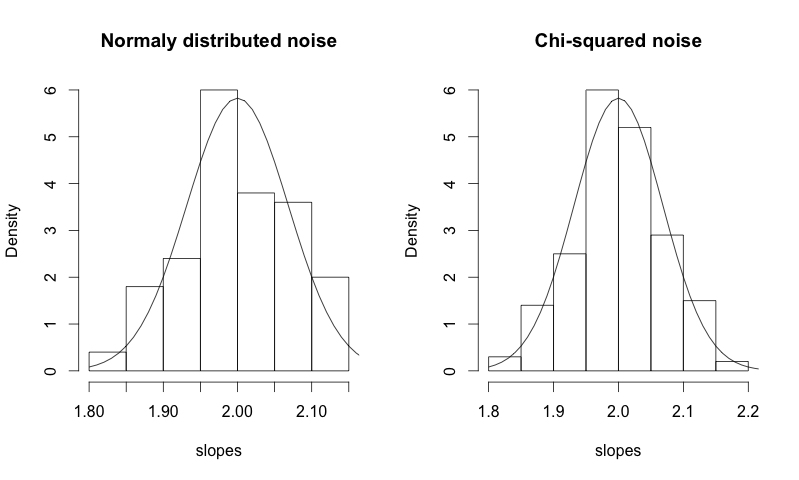
\includegraphics[scale = 0.55]{ex1_plot.png}

\pagebreak

\section*{Exercise 3}
%
a,b) The plots below both show an increase of number of passengers in the USA between 1949 and 1960 that seems nearly linear in time, however with strong seasonal fluctuations. Whereas the original plot shows increasing fluctuations over time, in the logarithmic plot the we observe steady fluctuations.

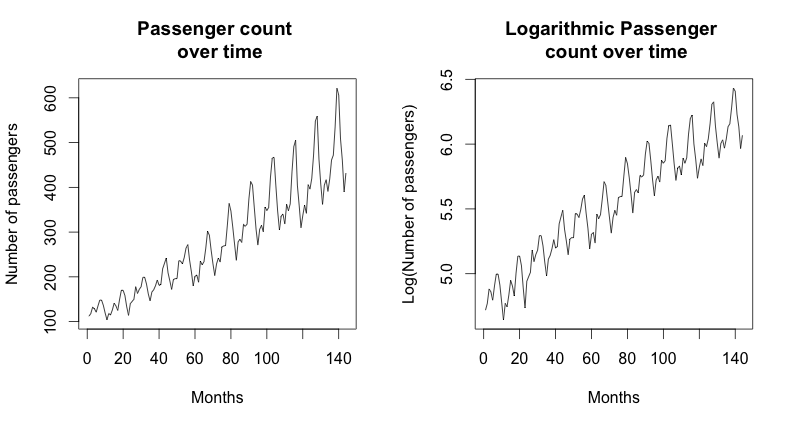
\includegraphics[scale = 0.5]{ex3_plot1.png}
\\
c) The intercept parameter is not only unnecessary but would violate our model assumptions. This is because we require the design matrix to be of full rank and the sum of indicator vectors for months is exactly the vector of ones, corresponding to the intercept. Adding the intercept column would cause the matrix to be rank deficient.
\\
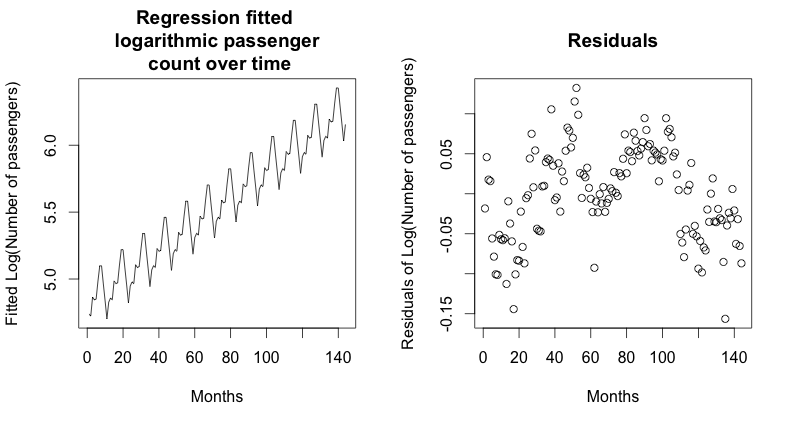
\includegraphics[scale = 0.5]{ex3_plot2.png}
\\
d) It seems that the assumption of uncorolated errors is violated here, as can be seen from the clusters in the residuals plot.

\end{document}

